
\section{Solution}
\label{sec:auswertung}

\subsection{Aufgabe 1} 

Das Minimum der Funktion 
\begin{equation}
    f(x) = x^2 - 2
\end{equation}
wird über das Intervallhalbierungsverfahren bei 
\begin{equation}
    x_\text{min} =  \num{-5.96046e-09}
\end{equation}
und über das Newton-Verfahren bei
\begin{equation}
    x_\text{min} = \num{1.13243e-14}
\end{equation}
gefunden.
Das wahre Minimum befindet sich bei $x=0$. Damit befindnen sich beide gefundenen Minimas in der Größenordnung der vorgegebenen Genauigkeit von $x_e = \num{1e-9}$.
Das Newton-Verfahren konvergiert schon noch einer Iteration. Dies liegt an der einfachen Form der Funktion: 
Da die erste Ableitung eine Gerade ist, führt die Tangente von jedem Startpunkt aus direkt zur Nullstelle. Bei analytischer Berechnung der Ableitungen wäre das Newton-Verfahren exakt.
Das Intervallhalbierungsverfahren konvergiert erst nach $60$ Schritten, dabei könnte es in diesem Fall mit einer nur geringfügig reduzierten Genauigkeit schon nach ca. $20$ Schritten konvergiert sein.

\begin{figure}
    \centering
    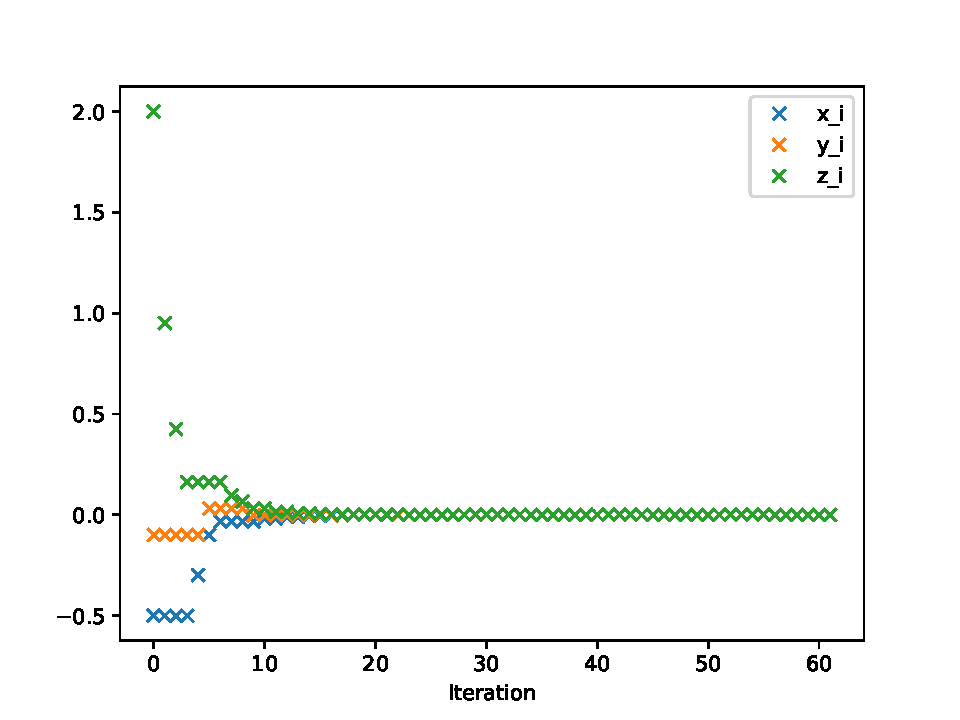
\includegraphics[width=.6\textwidth]{images/Halbierung.pdf}
    \caption{Werte des Intervallhalbierungsverfahren.}
\end{figure}

\begin{figure}
    \centering
    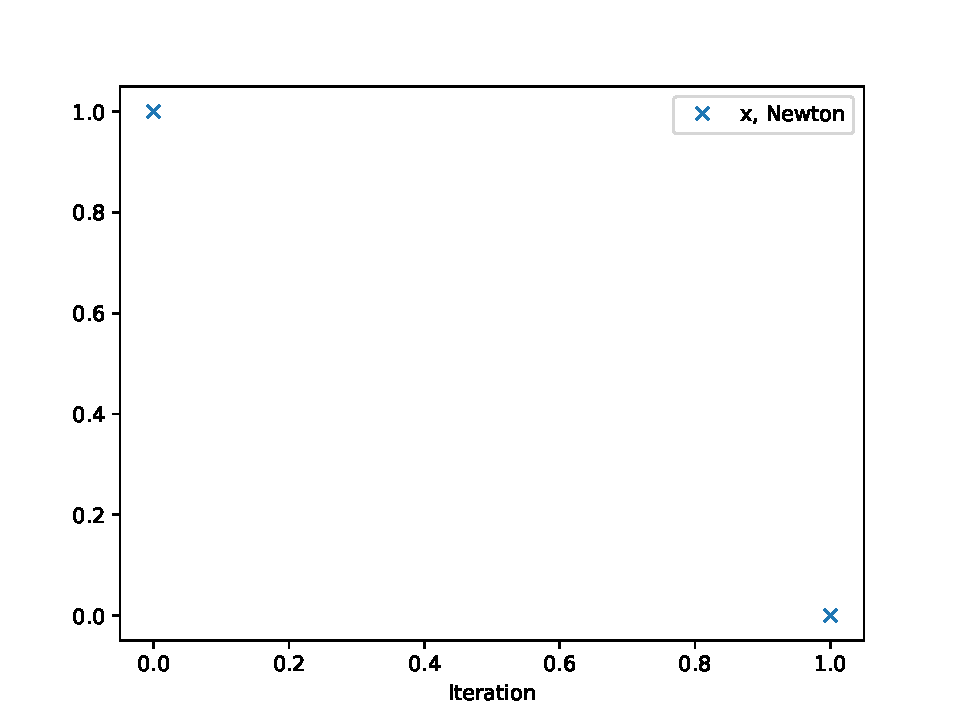
\includegraphics[width=.6\textwidth]{images/Newton.pdf}
    \caption{Werte des Newton-Verfahrens.}
\end{figure}